\section{Postgres: Restoring from PITR}
\label{app_pg_s1e1}

In this experiment we simluated data loss in a postgres database and restored the data with Point-in-time-Restore. 

Given that an attacker encrypts data files in a database in a ransomware attack, we assume complete data loss in the database. This can be simulated with a database (consisting of a single table) being dropped. This is because the security measures designed to mitigate such an attack work the same regardless of the state of the database.

\begin{figure}[h]
    \centering
    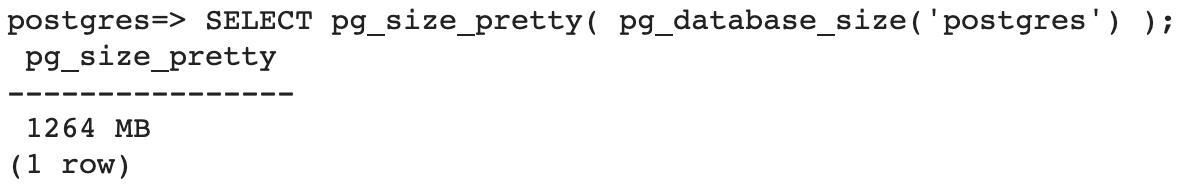
\includegraphics[width=\textwidth]{figures/postgres/postgres-1GB.png}
    \caption{The size of the inventory table}
    \label{fig:my_label}
\end{figure}

\begin{figure}[h]
    \centering
    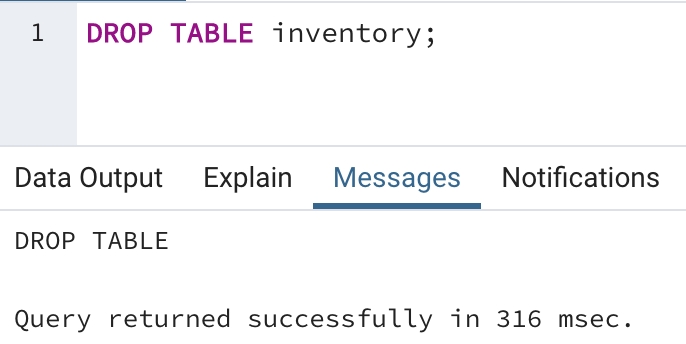
\includegraphics[scale=0.75]{figures/postgres/drop_table.png}
    \caption{Dropping the table}
    \label{fig:my_label}
\end{figure}

\begin{figure}[h]
    \centering
    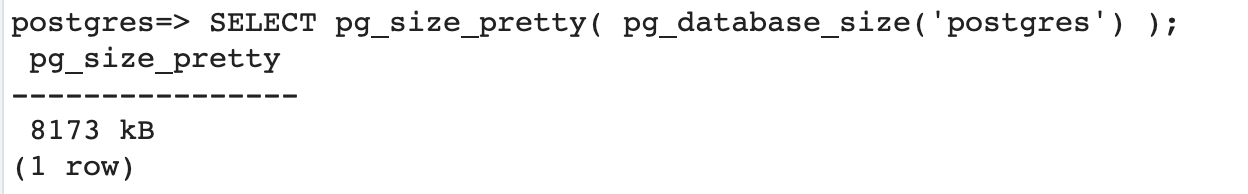
\includegraphics[width=\textwidth]{figures/postgres/postgres_size_post.png}
    \caption{The size of the inventory table after dropped table}
    \label{fig:my_label}
\end{figure}


The first security measure is also the simplest solution Azure provides for postgres databases: Point-in-time Restore (PITR). Though there are multiple ways to back up our database.

A point-in-time restore allows the database to be reverted back to a previous state where data has not been tampered with. The user specifies a point in time at which a copy of the database is made and used in the creation of a new managed database server. Such an operation is demonstrated in the following deployment of a restoration database.

\begin{figure}[H]
    \centering
    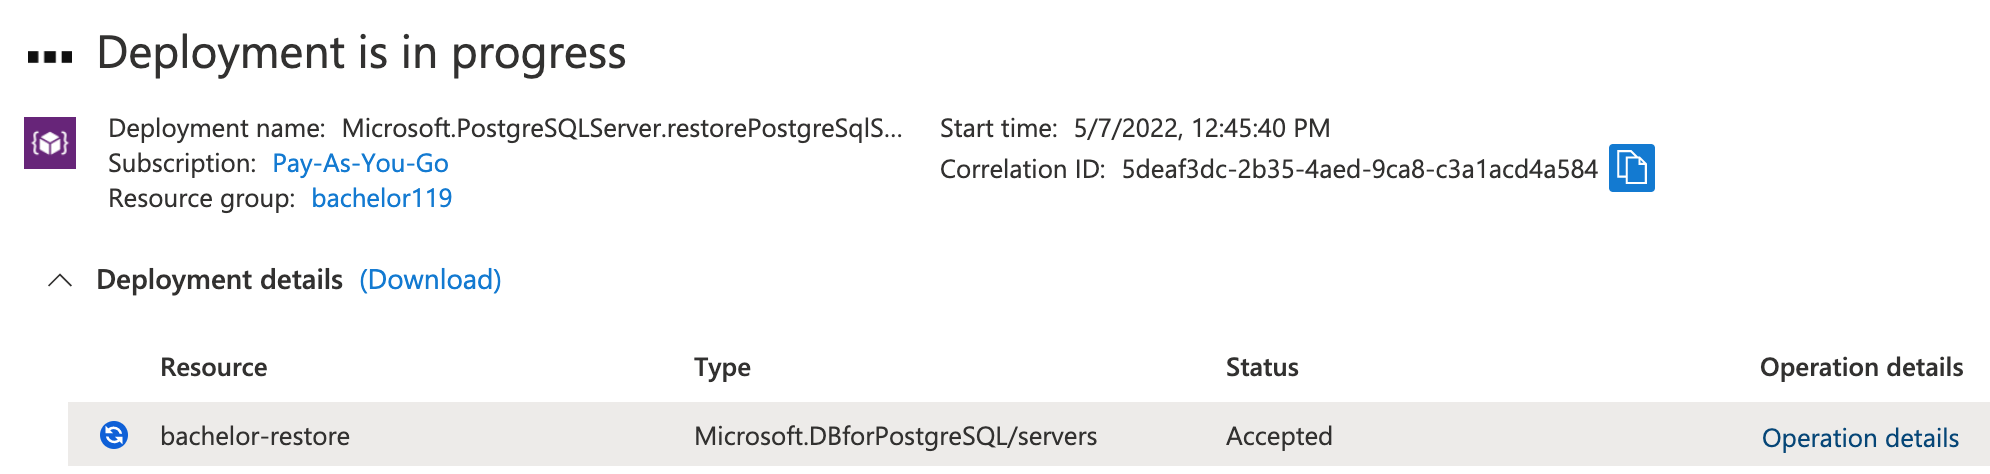
\includegraphics[width=\textwidth]{figures/postgres/restore_database.png}
    \caption{The restore operation took 31 minutes 27 seconds to complete}
    \label{fig:my_label}
\end{figure}

%This method is especially useful in cases of slow encryption that has been going on for a longer time before being detected.
%This is due to the option of salvaging the  encrypted parts of the database by restoring into a previous unencrypted state and setting together the puzzle pieces of the restored and the live database. 
This way one can recover to the most updated version of the database possible while removing all remnants of malicious activity.
%The estimated time of recovery depends on several factors including the database sizes, the transaction log size, the network bandwidth, and the total number of databases recovering in the same region at the same time. The recovery time varies depending on the the last data backup and the amount of recovery needs to be performed. It is usually less than 12 hours.

The policy for backup retention is dependent on the size of the server. Since we have a 7-day retention period set on the server and the server is no more than 4 TB the backup storage will retain 2 full backups, as well differential backups along with transaction logs from the point of the last full backup. Further information about how server size affects backup and restore policy can be found in the Azure docs for PostgreSQL single server.

%Servers with up to 16-TB storage will retain the full database snapshot, all the differential snapshots and transaction log backups in last 8 days.
%Another option is using the backup vault.
%Our performance tests show that the backup vault provides a performance boost compared to the point-in-time restore. 
%When RPO is of great importance and the operations of the business require handling hundreds of gigabytes of data the difference can be significant enough to make the vault a better suited solution for dealing with the encryption attack scenario.


